\section{Lezione del 27 ottobre}
Riprendiamo il discorso in cui affermiamo che Clique è in \textbf{NP} e in \textbf{NP-difficile} di cui è stata dimostrazione.

Quello che vogliamo vedere oggi è che la trasformazione di una formula $\phi$, dopo aver fatto la riduzione da 3Sat a Clique, in un grafo $G$ è una riduzione.
\subsection{Dimostrazione}
Per la dimostrazione si devono dimostrare le due direzioni:
\begin{enumerate}
\itemsep1pt\parskip0pt\parsep0pt
    \item \textbf{Dato un assegnamento di verità della formula, si costruisce la clique} Dato un assegnamento che rende vera la formula $\phi$ (che ha $k$ clausole), bisogna costruire una clique per il grafo $G$ che abbia $k$ vertici.\\ Ciascuna clausola $c_r$ ha almeno un letterale $l_i^r$ che ha valore assegnato pari a $1$. Ciascun letterale corrisponde ad un vertice $v_i^r$ (si ha che $l_i^r \to v_i^r$). Si costruisce l'insieme $V'$ di vertici per ogni letterale $l_i^r$ vero (e quindi per ogni clausola $c_r$). Si dimostra che $V'$ è una clique. \\ Infatti per ogni coppia $v_i^r, v_j^s \in V'$ con $r \neq s$, abbiamo che $(v_i^r, v_j^s) \in E$ e entrambi i letterali sono consistenti, ovvero uno non è derivato dalla negazione di una variabile presa come positiva nell'altro letterale.
    \item \textbf{Data una clique, si costruisce l'assegnamento di verità della formula} Si supponga che $G$ abbia una clique $V'$ di dimensione $k$; bisogna quindi far vedere che $\phi$ è vera.\\ Per costruzione $V'$ ha esattamente un solo vertice per ogni clausola ($v_i^r$ per la clausola $c_r$). Quindi per ogni clausola $c_r$ si assegna al letterale corrispondente $l_i^r$ il valore $1$. Sapendo che il letterale complementare $l_i^r$ non verrà usato per rendere vera una clausola in quanto il vertice $v_i^r$ non è collegato con un arco ad un vertice che rappresenta il complemento di $l_i^r$. Quindi si riesce a costruire un'assegnamento di verità consistente per $\phi$, ovvero ogni variabile viene presa come $x_i = 0$ oppure come $x_i = 1$, non utilizzando mai entrambi i valori.
\end{enumerate}
La struttura dimostrativa è sempre la stessa, si hanno infatti due direzioni ogni volta, quindi sarà sempre una situazione dove $\displaystyle x_{\in I_A} \to f_{\in I_B}(x)$ con riduzione polinomiale messa nel modo $A \leq_p B$. Ora ci serve mostrare che se x appartiene al linguaggio A (cioè ammette risposta affermativa) allora f(x) appartiene al linguaggio di B. Lo possiamo scrivere come $x \in L_A \to f(x) \in L_B$.

Si può fare la dimostrazione che Clique $\leq_p$ Vertex Cover, avendo visto un esempio simile Independent set $\leq_p$ Vertex Cover (e viceversa). \hfill

Possiamo osservare che se $A \leq_p B$ e $A, B \in$ NP-completi $\to B \leq_p A$.\hfill
\subsection{Problemi di ottimizzazione}
Dato un problema $\Pi$ e un'istanza $x$, l'ottimo su $x$ di $\Pi$, indicato come $opt()$, è il valore numerico che quantifica la soluzione ottimale (tra tutte quelle ammissibili), ovvero quella che massimizza o minimizza una certa funzione costo. Il costo di una soluzione ammissibile su $x$ calcolato da un algoritmo $A$ per il problema $\Pi$ viene indicato con $A(x)$. Tra tutte le soluzioni ammissibili di $\Pi$, sicerca la soluzione che massimizza o minimizza un costo. 

\textbf{Algoritmo $\varepsilon$-approssimato} per un problema $\Pi$ di ottimizzazione è un algoritmo $A$ polinomiale tale che restituisce una soluzione ammissibile che dista da quella ottima di un fattore costante $\varepsilon$. 
\begin{itemize}
    \item Se $\Pi$ è un problema di minimo allora: $A(x) \leq \varepsilon \cdot opt(x)$ dove $\varepsilon > 1$.
    \item Se $\Pi$ è un problema di massimo allora: $A(x) \geq \varepsilon \cdot opt(x)$ dove $0 < \varepsilon < 1$, in questo caso notiamo che il valore di $\varepsilon$ viene dato per mezzo di una frazione.
\end{itemize}
La caratteristica della $\varepsilon - approssimazione$ è che vado a trovare un $A$ che lavora in tempo polinomiale che risolve in modo approssimato un problema tendenzialmente in NP-completo. \\
Il fattore $\varepsilon$, che è una costante numerica che non dipende dall'input, funge da \textbf{garanzia} sulla distanza dal costo della soluzione trovata da quella ottimale. Ricordiamo che $A(x)$ è il costo della soluzione ammissibile calcolata da un algoritmo A.

Quando si parla \textbf{tasso di approssimazione (approximation ratio)} ci sono diverse approssimazioni. Quello che però identifica sono le prestazioni di un algoritmo di approssimazione possono essere valutate mediante: 
\[
    \max
    \begin{Bmatrix}
    \displaystyle \frac{A(x)}{opt(x)}, \frac{opt(x)}{A(x)}
    \end{Bmatrix}
    \leq r
\]
Dove
\begin{itemize}
    \itemsep1pt\parskip0pt\parsep0pt
    \item $A(x)$: soluzione approssimata
    \item $opt(x)$: soluzione ottima
    \item $r$: fattore di approssimazione (utilizzato al posto di $\varepsilon$ al fine di avere sempre un valore intero).
\end{itemize}

Non tutti i problemi NP-completi ammettono una $r$-approssimazione, per $r$ costante. Infatti il tasso di approssimazione può essere espresso mediante una funziona $\rho(n)$ che dipende dalla dimensione dell'input ($|x| = n$). La dimensione del problema influisce sulla capacità di approssimare il problema, in poche parole l'approssimazione peggiora all'aumentare delle dimensioni del problema.

\begin{figure}[H]
    \centering
    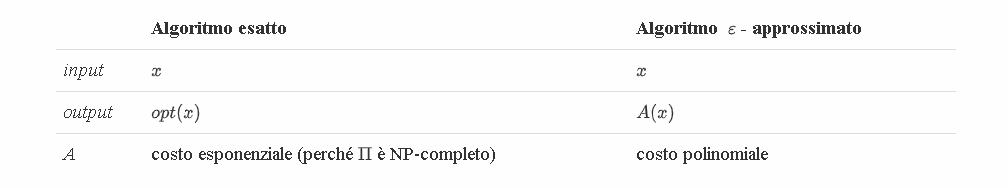
\includegraphics[scale = 0.5]{imm/algoritmo_esatto.PNG}
\end{figure}

$\exists$ un algoritmo $A$ polinomiale per Vertex Cover 2-approssimante trovandomi ad affrontare $\displaystyle \frac{A(x)}{opt(x)}\leq 2$.
Per trovare $\varepsilon$, si fornisce un'euristica $A$ per Vertex Cover, cioè un modo per ottenere in tempo polinomiale una copertura di vertici per $G$, e poi si prova a dimostrare, senza conoscere $opt(x)$ (per ogni input $x$), che $\displaystyle \frac{A(x)}{opt(x)} \leq \varepsilon$ e si ha una $\varepsilon$-approssimazione.\\
Pur non conoscendo l'ottimo è possibile fare una stima del valore del rapporto, perché è possibile immaginare come potrebbe essere l'ottimo in funzione dell'input.\\

\subsection{Vertex Cover Approx}
Inventare un'euristica polinomiale per calcolare una copertura per un grafo (Vertex Cover) con $G = (V. E)$. 
Cerco un $A$ che calcoli in tempo polinomiale una soluzione ammissibile, ovvero una copertura di vertici del grafo. Si sceglie che $A$ non deve essere un \textit{algoritmo greedy}. Prendo quindi un arco del grafo $e=(u,v)\in E$. Inizio a costruire una copertura $C$, all'inizio vuota ($C=\emptyset$), che ora diventa, aggiungendo i due vertici: $C=C\cup\{u,v\}$\\
Inoltre rimuovo dall'insieme degli archi $E$ tutti gli archi che hanno un estremo nell'attuale copertura $C$, e quindi nel nostro caso in $u$ o $v$. La copertura $C = \varnothing$, risulta la mia soluzione ammissibile che inizialmente la troviamo vuota. Finché $E = \varnothing$.
L'algoritmo restituisce: $A(x) = 2 \times $numero di archi scelti in $E$.

\begin{lstlisting}
Approx(G)
C  := null 
E' := archi di G
while E' != null do 
    let (u,v) appartenente a E'
    C := C union {u,v}
    per ogni (u,z) in E', (v,z') in E'
        rimuovi (u,z), (v,z') da E' 
return C
\end{lstlisting}

È un algoritmo polinomiale nella dimensione di $G$ ($|V|, |E|$).

È quindi una 2-approssimazione in quanto al massimo posso prendere il doppio dei vertici per fare la copertura, infatti, per costruzione, seleziono ogni volta archi che non hanno estremi in comune. Per ognuno di questi archi scelti devo prendere i due estremi, quindi ho $2\cdot k$ vertici in $C$ per $k$ archi e quindi: $A(x)=2\cdot k$.
Ma di $opt(x)$ so che nel casi migliore prende esattamente un estremo per ogni scelto dall'algoritmo, e quindi per archi che non hanno estremi in comune. Quindi nel caso migliore: $opt(x)\geq k$. Ma dato che stiamo cercando di minimizzare, quindi $k$ è il \textit{lower bound} vale quindi: $\displaystyle\frac{A(x)}{opt(x)}\leq\frac{2k}{k}\leq 2$.